\section{Bedingte Ausführung}

\begin{frame}{Bedingte Ausführung}
\centering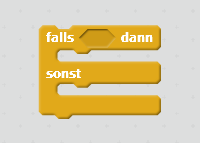
\includegraphics[scale=1.0]{images/wenndann}
\end{frame}

\begin{frame}[fragile]{Bedingte Ausführung}
Umgangssprachlich:\\ Wenn (if) eine \textcolor{red}{Bedingung} True ist, dann führe Programmcode 1 aus, andernfalls (else) Programmcode 2\\

\begin{lstlisting}
if Bedingung == True:
	# Programmcode 1 
else:
	# Programmcode 2 
\end{lstlisting}

\begin{lstlisting}
zahl = int(input("Zahl: "))

if zahl > 10:
	print("Die Zahl ist > 10.")
else:
	print("Die Zahl ist <= 10.")
\end{lstlisting}
\end{frame}

\begin{frame}[fragile]{Bedingte Ausführung}
Schreibe ein Programm, das eine Eingabe einliest und speichert mit input(''Wetter: '').
Falls die Eingabe ''Schnee'' lautet, gebe ''Es ist Winter'' aus. Andernfalls gebe ''Noch einmal Glück gehabt'' aus.
\pause{}
\begin{lstlisting}
inp = input("Wetter: ")
if inp == "Schnee":
    print("Es ist Winter")
else:
    print("Noch einmal Glück gehabt")
\end{lstlisting}
\end{frame}

\begin{frame}[fragile]{Mehrfach bedingte Ausführung}
Umgangssprachlich:\\ Wenn (if) eine \textcolor{red}{Bedingung1} True ist, dann führe Programmcode 1 aus, \\falls nicht, dann prüfe (elif) ob \textcolor{red}{Bedingung2} True ist, dann führe Programmcode 2 aus, \\andernfalls (else) Programmcode 3.\\

\begin{lstlisting}
if Bedingung == True:
    # Programmcode 1
elif Bedingung2 == True:
    # Programmcode 2
else:
    # Programmcode 3
\end{lstlisting}
\end{frame}


\begin{frame}[fragile]{Mehrfach bedingte Ausführung - Beispiel}
\begin{lstlisting}
zahl = int(input("Zahl: "))

if zahl > 10:
    print("Die Zahl ist > 10.")
elif zahl > 5:
    print("Die Zahl ist > 5 und <= 10.")
else:
    print("Die Zahl ist <= 5.")
\end{lstlisting}
\end{frame}


\begin{frame}[fragile]{Bedingte Ausführung}
Ergänze das zuvor erstellte Programm so, dass nicht nur der Fall ''Schnee'' abgefragt wird, sondern auch ''Sonne''. Bei Eingabe Sonne verwende print(''Ein paar letzte Sonnenstrahlen'') und  print(''Genieße solange wie möglich'').
\pause{}
\begin{lstlisting}
inp = input("Wetter: ")
if inp == "Schnee":
    print("Es ist Winter")
elif inp == "Sonne":
    print("Ein paar letzte Sonnenstrahlen")
    print("Genieße solange wie möglich")
print("Noch einmal Glück gehabt")
\end{lstlisting}
\end{frame} 


\begin{frame}[fragile]{Schachtelung}
\begin{itemize}
	\item Bedingungen und Schleifen (dazu später) können beliebig oft ineinander geschachtelt werden
	\item Erkennbar durch Einrückungen
	\item Beachte Logik
	\item Zu viele Schachtelungen führen zu Unübersichtlichkeit \texttt{=>} schlechter Code
\end{itemize}
\end{frame}


\begin{frame}[fragile]{Schachtelung bedingter Ausführungen}

\begin{lstlisting}
zahl = int(input())

if zahl < 10:
    if zahl < 5:
	     print("Die Zahl ist < 5")
	else:
		 print("Die Zahl ist >= 5 und < 10")
else:
	print("Die Zahl ist > 10")
\end{lstlisting}
\end{frame}


\begin{frame}{Bedingte Ausführung - Übung}
Aufgabe: Hundealter in Menschenalter\\
Bei kleinen Hunden entspricht das erste Lebensjahr etwa 20 Menschenjahren. Das zweite entspricht 8 Jahren und alle weiteren Hundejahre entsprechen jeweils 4 Menschenjahren. Bei einem 5-jährigen Hund rechnest du also: 20 + 8 + 4 + 4 + 4 = 40. Fünf Hundejahre wären demnach etwa 40 Menschenjahre.\\
\end{frame}
\begin{frame}{Bedingte Ausführung - Übung 1}
Kurz:
\begin{itemize}
\item 1. Hundejahr $=$ 20 Jahre
\item 2. Hundejahr $=$ 28 Jahre
\item Über 2 Jahren $= 20 + 8 + (Alter - 2)  *  4$ Jahre
\end{itemize}
Aufgabe:
Es soll ein Programm geschrieben werden, das mit input() nach dem Alter fragt (nur positives Hundealter), mit bedingter Ausführung das Menschenalter ermittelt und ausgibt.
\begin{itemize}
	\item input(''Alter des Hundes: '')
	\item bedingte Ausführung
	\item print(''Das entspricht ca. ??? Jahren.'')
\end{itemize}

\end{frame}

\begin{frame}[fragile]{Bedingte Ausführung - Übung}
\begin{exampleblock}{Lösung}
\begin{lstlisting}
alter = int(input("Alter des Hundes: "))
if age == 1:
	print("Das entspricht ca. 20 Jahren.")
elif age == 2:
	print("Das entspricht ca. 28 Jahren.")
else:
	human = 28 + (age -2)*4
	print("Das entspricht ca. " + str(human) + " Jahren.")
\end{lstlisting}
\end{exampleblock}
\end{frame}



